% ----------------------------------------------------------------------
% Template VERIFICA
% ----------------------------------------------------------------------
% 2020 di d!egofantinelli at jazzmagus@gmail.com
% ----------------------------------------------------------------------

% ---------------------------------- Preambolo
\documentclass[11pt, a4paper]{exam}
\usepackage[T1]{fontenc}
\usepackage{mdframed}
%\usepackage{nicefrac}
%\usepackage[applemac]{inputenc}
%\usepackage[utf8]{inputenc}
\usepackage[italian]{babel}
\usepackage[margin=1.3in]{geometry}
\usepackage{amsmath,amssymb}
\usepackage{multicol}
\usepackage{graphicx}
\usepackage{tikz}
\usepackage{upquote}
\usepackage{caption}
%\usepackage{fancyhdr}
\usepackage{float}


\renewcommand{\questionshook}{%
    \setlength{\leftmargin}{0pt}%
}
\renewcommand{\choiceshook}{%
    \setlength{\leftmargin}{20pt}%
}


% ---------------------------------- Intestazione
\newcommand{\class}{\huge {Verifica di Recupero di Matematica}}
\newcommand{\term}{1� Quadrimestre}
\newcommand{\examnum}{Verifica numero: 02 | 02}
\newcommand{\examdate}{03 marzo 2021}
\newcommand{\timelimit}{50 minuti}

\CorrectChoiceEmphasis{\color{red}}
\SolutionEmphasis{\color{red} \footnotesize}
\renewcommand{\solutiontitle}{\noindent\textbf{Soluzione:}\par\noindent}
% ---------------------------------- Intestazione

\pagestyle{headandfoot}
\firstpageheader{IIS "G. A. Remondini" - Bassano del Grappa (VI)}{}{\examdate}
\runningheader{\footnotesize VERIFICA di Recupero di MATEMATICA}{}{Classe 4\string^QA}
\runningheadrule

\firstpagefooter{}{}{pag. \thepage\ di \numpages}
\runningfooter{}{}{pag. \thepage\ di \numpages}
\runningfootrule

% ---------------------------------- Punteggi
\pointpoints{punto}{\em punti}
\pointformat{[{\footnotesize \thepoints}]}
\bonuspointpoints{punto bonus}{\em punti bonus}
\bonuspointformat{[{\footnotesize \thepoints}]}
\pointsinrightmargin
\setlength{\rightpointsmargin}{.2cm}
\chqword{Esercizio}
\chpword{Punti}
\chbpword{Punti Bonus}
\chsword{Punteggio}
\chtword{Totale}

\begin{document}

% ---------------------------------- Title Page
\begin{center}
\rule[2ex]{\textwidth}{0.5pt}\\
{\huge{\bf \class}}\\[12pt]
%{\huge - Recupero Primo Quadrimestre -}\\[8pt]
\rule[2ex]{\textwidth}{0.5pt}\\
\end{center}
\vspace{3cm}
\begin{tabular*}{\textwidth}{l @{\extracolsep{\fill}} r @{\extracolsep{6pt}} l}
\textbf{} & \textbf{Nome e Cognome:} & \makebox[2.5in]{\hrulefill}\\
\textbf{} &&\\
\textbf{} & \textbf{Classe:} & \makebox[2.5in]{\Large{\bf 4 \string^ QA}}\\
\textbf{} &&\\
\textbf{} & Tempo a disposizione: & \makebox[2.5in]{\timelimit}
\end{tabular*}\\[3cm]

\vspace{5cm}
% ---------------------------------- Avvertenze

\noindent
%\rule[2ex]{\textwidth}{0.2pt}
\textbf{Avvertenze}:
\begin{itemize}
	\item La presente Verifica di Recupero - che viene somministrata in modalit� DDI - contiene \numquestions \; quesiti, per un totale di \numpoints \;punti;
	\item La webcam dovr� rimanere accesa per tutto il tempo della verifica (\timelimit), salvo impossibilit� concrete di connessione; il microfono rester� spento e verr� acceso soltanto per chiarimenti e domande, che saranno consentite negli ultimi 20 min di prova.
	\item E' vietato l'utilizzo di calcolatrici scientifiche, smartphone, tablet e altri dispositivi digitali, nonch� la consultazione di testi, appunti e siti web.

\end{itemize}
%\rule[2ex]{\textwidth}{0.2pt}
\vfill
\newpage

% ===================================== Esercizi

%\printanswers

\begin{questions}

% ------------------------------------- Esercizio 1
\addpoints
\question
Determina le soluzioni delle seguenti espressioni di secondo grado:\\
\begin{parts}
\part[5]
\(\dfrac{4}{3}x^2 - \dfrac{1}{4} = 0\)\\
\fillwithdottedlines{0.5in}
{\footnotesize
\begin{solution}
	\(x_1 = \dfrac{\sqrt{3}}{4}; \, x_2 = -\dfrac{\sqrt{3}}{4}\)
\end{solution}
}
\vspace{.75cm}

\part[5]
\(x^2 + 8x + 12 = 0\)\\
\fillwithdottedlines{0.75in}
{\footnotesize
\begin{solution}
	\(x_1 = -2; \, x_2 = -6 \)
\end{solution}
}
\end{parts}
\vspace{.5cm}

% ------------------------------------- Esercizio 2

\addpoints
\question [6]
Risolvi la seguente equazione di secondo grado e utilizza le soluzioni per fattorizzare il trinomio: \[2x^2 + 3x - 2 = 0 \]
\fillwithdottedlines{0.75in}

{\footnotesize
\begin{solution}
	\(x_1 = -2 \quad x_2=\dfrac{1}{2}\) 
\end{solution}
}
\pagebreak
% ------------------------------------- Esercizio 3
\addpoints
\question [8] Data la seguente funzione quadratica \[y = -x^2 + 4x - 12\] Disegnane il grafico dopo averne determinato le coordinate  dei punti di intersezione con gli assi e quelle del Vertice. \\

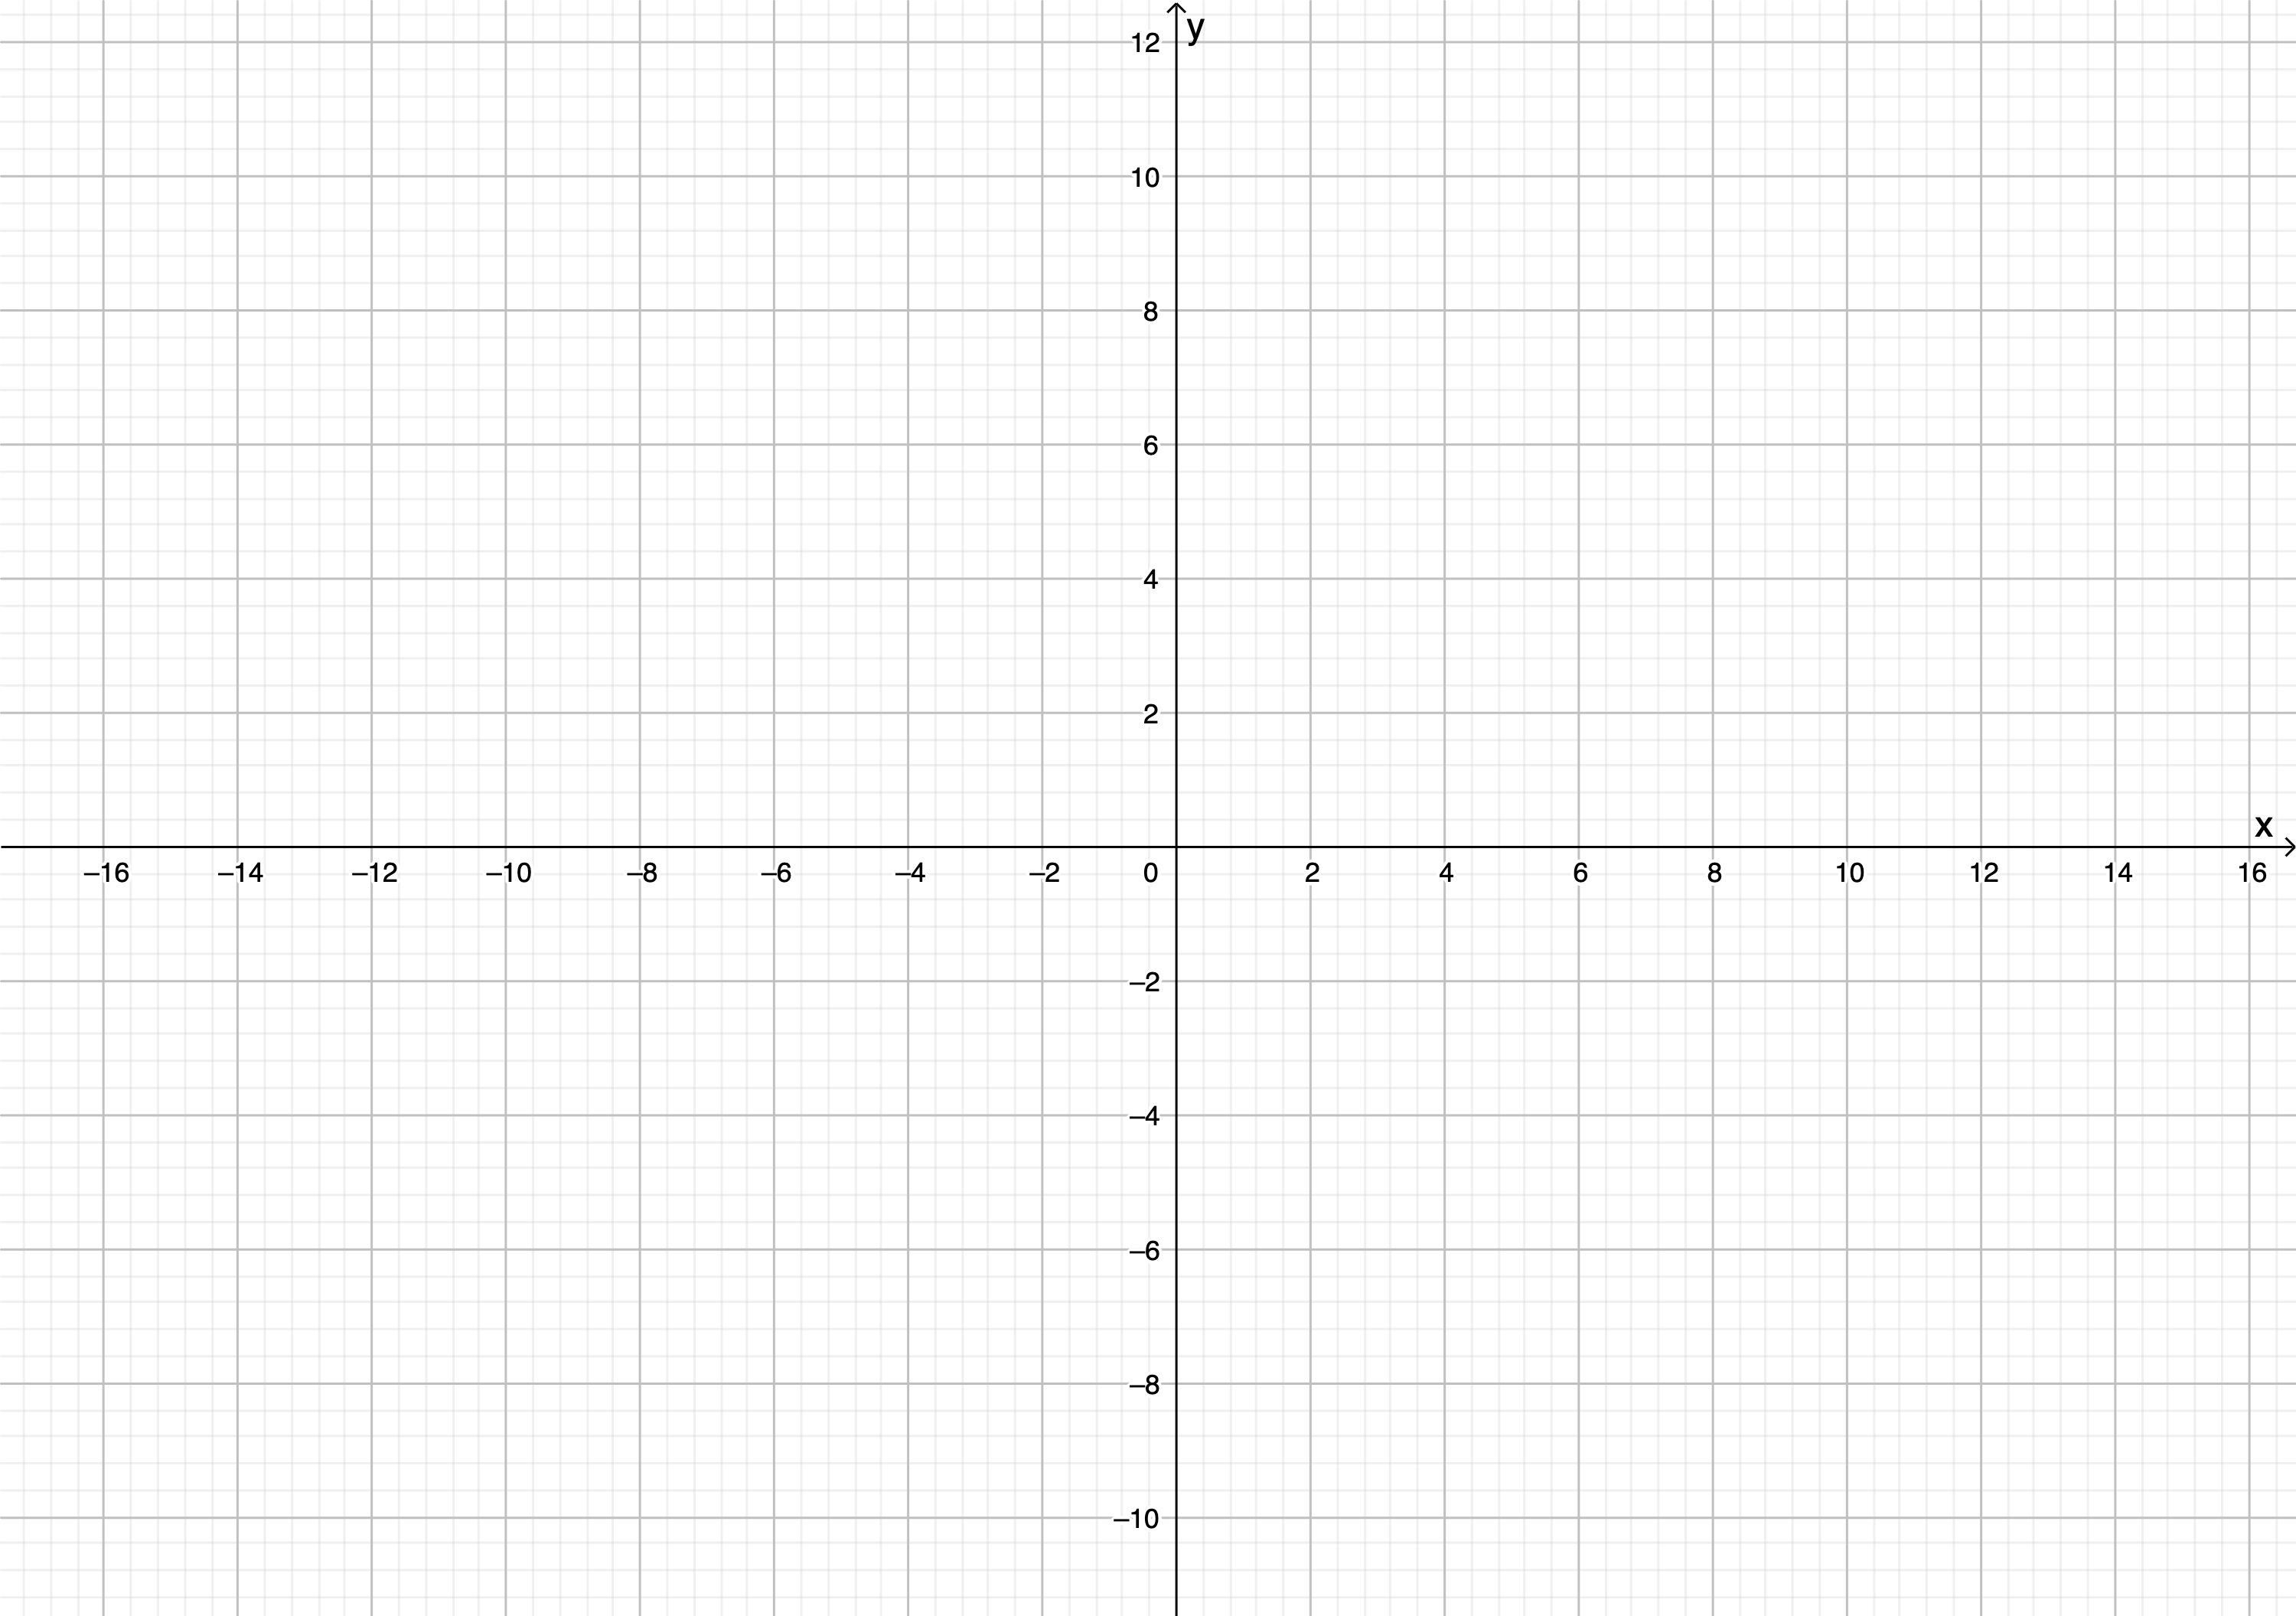
\includegraphics[width=\textwidth]{grafico_empty}
%\fillwithlines{1in}
\pagebreak
% ------------------------------------- Esercizio 4
\addpoints
\question [6]
Quello in figura � il grafico di una determinata funzione di secondo grado del tipo \(y = ax^2 + bx + c\);\\
Ricostruisci l'equazione della funzione aiutandoti con i punti evidenziati:\\
\vspace{8pt}

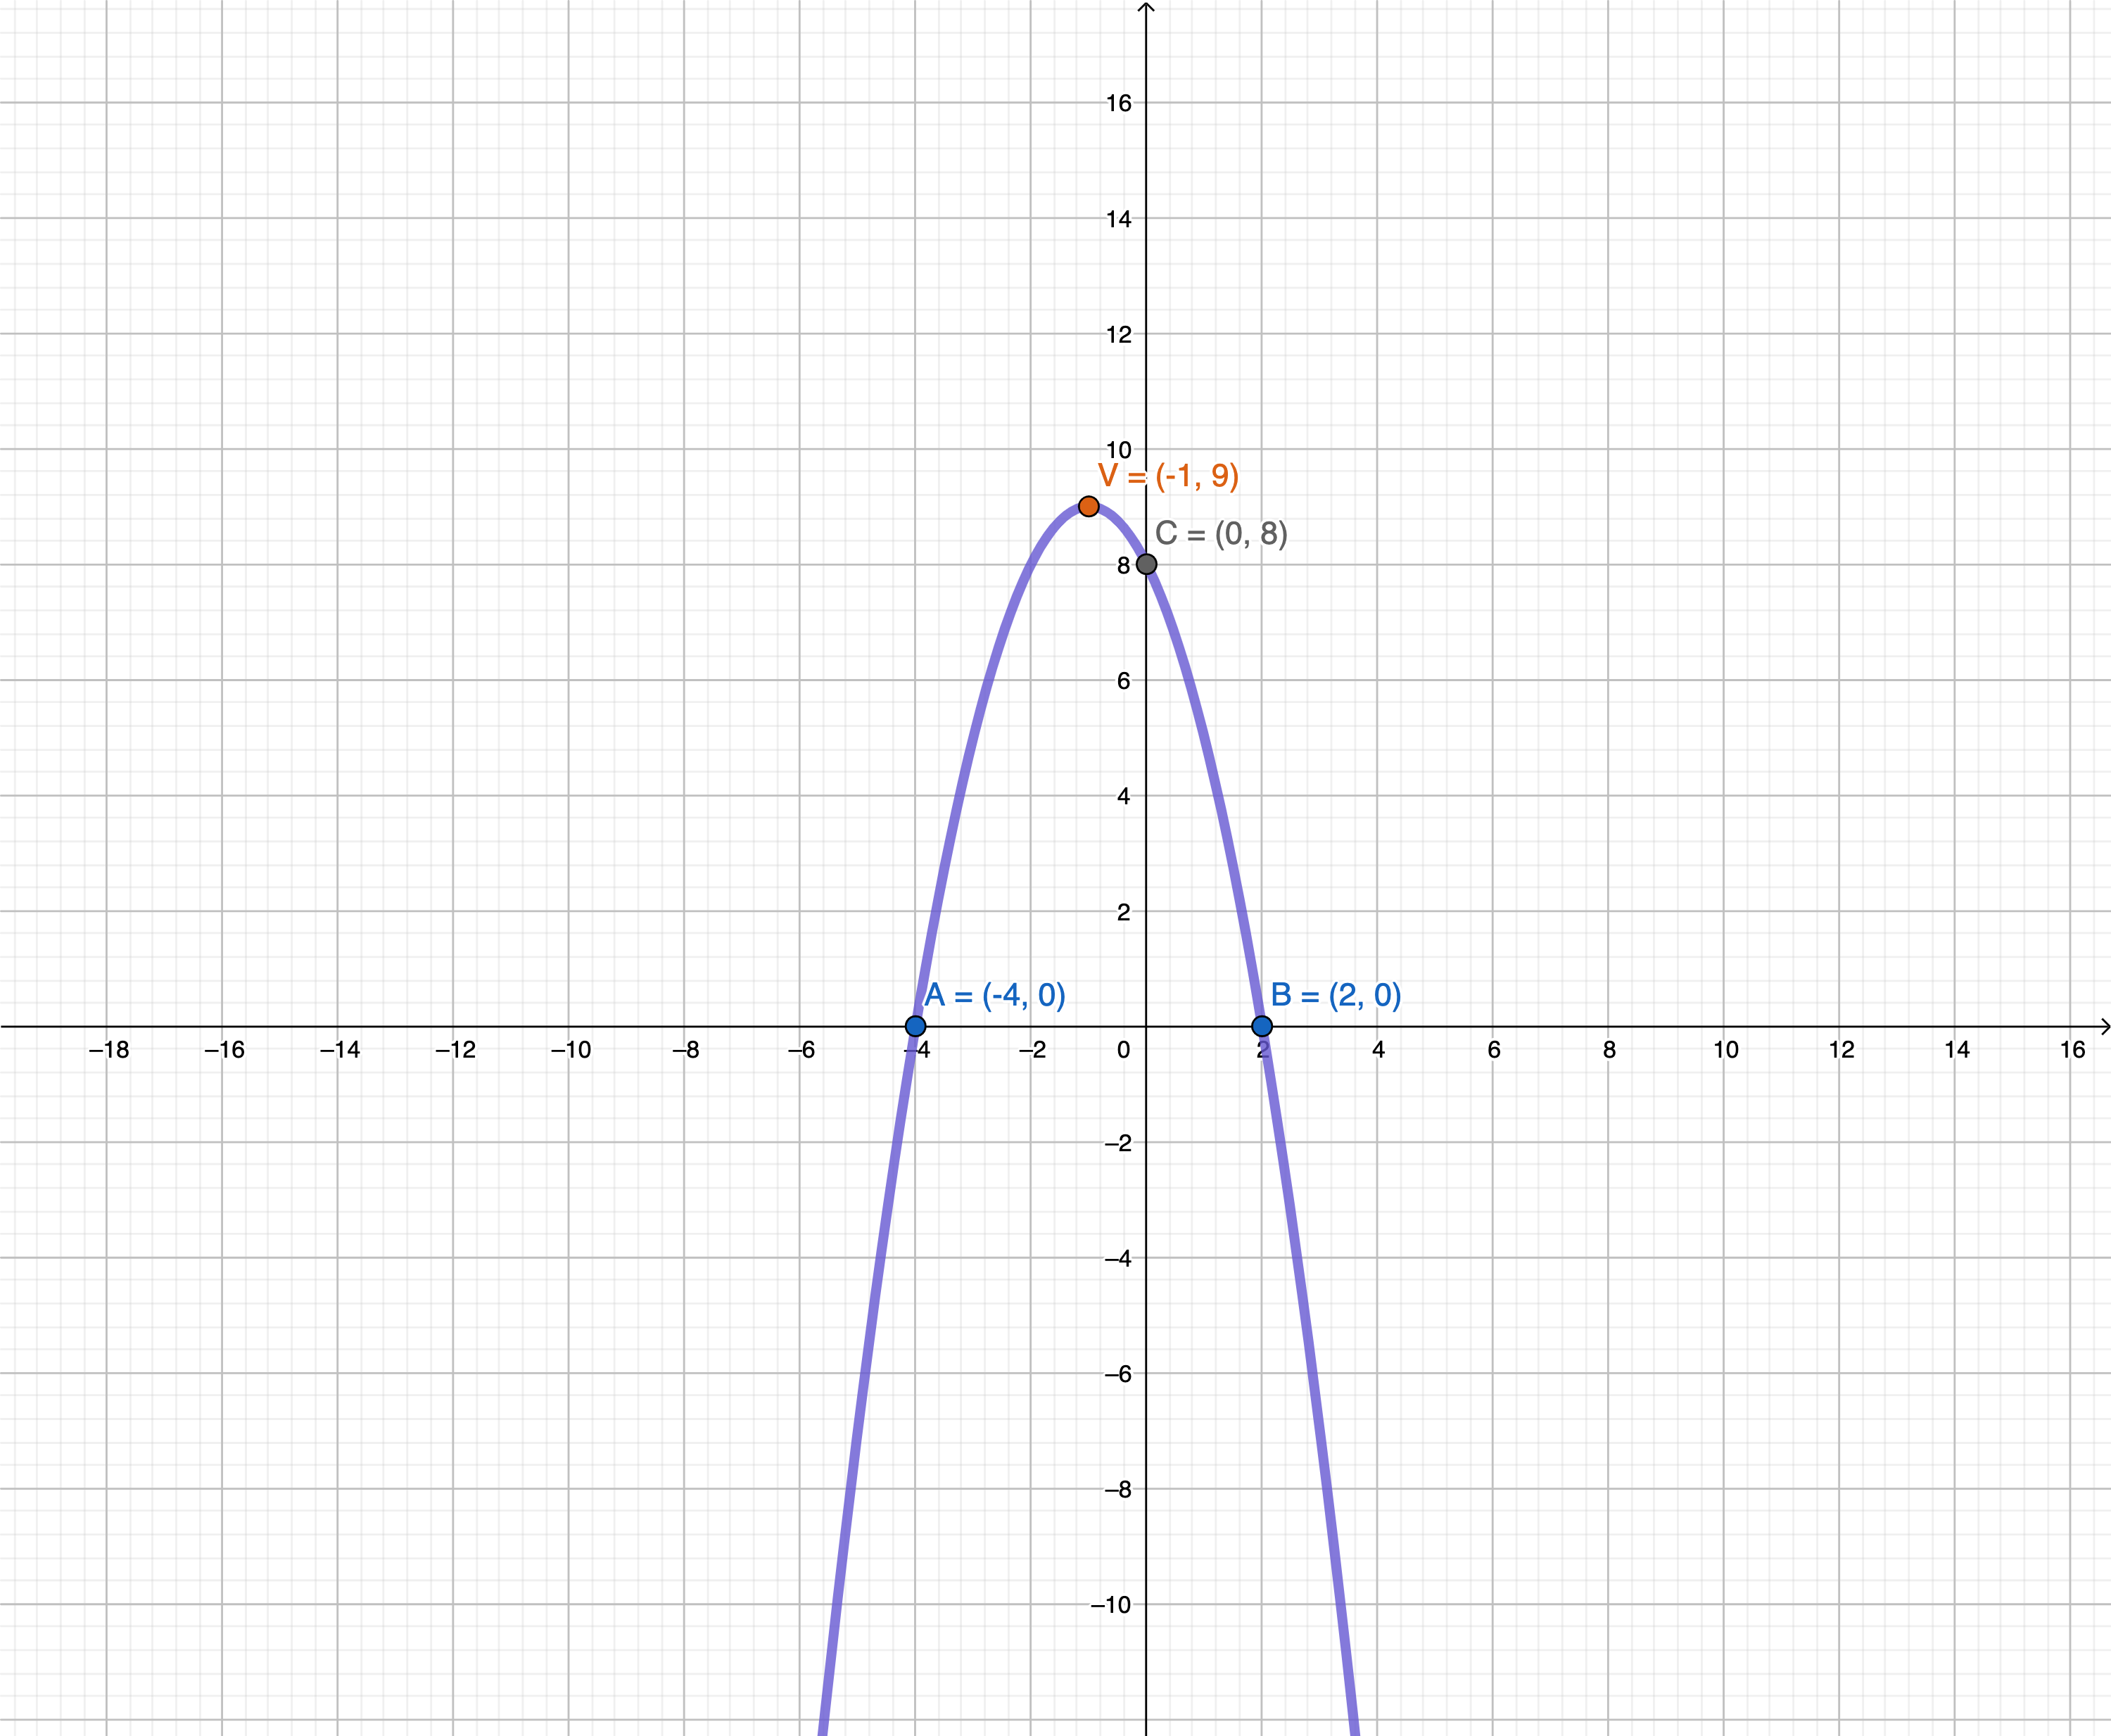
\includegraphics[width=\textwidth]{graph_ex3}\\

\fillwithdottedlines{0.75in}
{\footnotesize
\begin{solution}	
	\(y = x^2 + 4x - 12\)
\end{solution}
}

\end{questions}
\vfill

%\pagebreak
\hrule
\begin{center}
{\bf Tabella dei punteggi}
\vspace{10pt}

\combinedgradetable[h][questions]
\end{center}
\vspace{4pt}
\footnotesize La sufficienza � fissata a 20 punti, ma potr� subire delle modifiche in fase di correzione, al fine di garantire la validit� della prova anche nel caso in cui si riscontrino prestazioni della classe sensibilmente lontane dalla media-classe stimata.

\end{document}
